%  NOTE: Please make sure to completely fill out the \def parts in meta-data.tex!

\section*{Preface}
Some room for acknowledgements.

\newpage \thispagestyle{empty} \strut
\newpage \pagenumbering{arabic}

\title{\thesistitle{}}
\author{\yourname}

\maketitle % Yes, again

\begin{abstract}

\end{abstract}

\section{Introduction}



\section{Related Work}



\section{Experimental Setup}



\subsection{Data}
\hfill
\subsubsection{Source}

The data consists of $405$ EAF-files (ELAN Annotation Files) gathered by the Institute for German Sign Language and Communication of the Deaf at Hamburg University \cite{prillwitz2008dgs}. These files consist of a total of $50$ hours of annotated recordings spanning a wide range of narrations regarding the cultural aspects of the deaf community. The interviews were conducted using a peer-to-peer procedure, where participant change roles according to the conversation \cite{prillwitz2008dgs}. During a discussion $2$ German Sign Language or Deutsche Gebärdensprache (DGS) signers conversed. Each conversation consisted of a standardized interview covering linguistical and social data \cite{deaf_areas}. Following this conversation a spontaneous conversation on a given topic was held while the participants were encouraged to use as much basic vocabulary as possible \cite{deaf_areas}. In the EAF-files the signers are annotated as either Speaker A or Speaker B. The data was collected between January $2010$ and December $2011$  by videotaping $330$ participants from all $16$ Federated States (Bundesländer). The recordings were conducted using a mobile field lab in:

\begin{itemize}
  \item Areas with a relatively high deaf population density (deaf schools, deaf centres, and deaf institutes). \cite{age_data_hamburg} \cite{deaf_areas}
  \item The catchment areas of the former Schools for the Deaf.\cite{age_data_hamburg} \cite{prillwitz2008dgs}
  \item Areas which were easy to reach from surrounding rural communities. \cite{age_data_hamburg} \cite{deaf_areas}
  \item Areas that were suspected of having a distinct dialect. \cite{age_data_hamburg} \cite{prillwitz2008dgs}
\end{itemize}

 The data was collected by representatives of the local deaf community to take into account the regional varieties of DGS \cite{deaf_areas}. As can be seen in \autoref{fig:bundeslander} the data was sampled from participants across different age groups \cite{age_data_hamburg}. 


% Age category figure
\pgfplotstableread[row sep=\\,col sep=&]{
    interval & carT & carD \\
    18--30     & 12.1  & 12.4  \\
    31--45     & 13.6 & 13.9  \\
    46--60   & 12.7 & 12.4 \\
    61+   & 11.5 & 11.2 \\
    }\mydata

\begin{figure}[h]
\begin{tikzpicture}
    \begin{axis}[
            ybar,
            bar width=.6cm,
            width=.8\textwidth,
            height=.5\textwidth,
            legend style={at={(0.5,1)},
                anchor=north,legend columns=-1},
            symbolic x coords={18--30,31--45,46--60,61+},
            xtick=data,
            nodes near coords,
            nodes near coords align={vertical},
            ymin=0,ymax=25,
            xlabel={\/Age categories},
            ylabel={\/Percentage of participants (\%)},
        ]
        \addplot table[x=interval,y=carT]{\mydata};
        \addplot table[x=interval,y=carD]{\mydata};
        \legend{Male, Female}
    \end{axis}
    
\end{tikzpicture}
\caption{Showing the percentage of participants per age , divided into both the Male (shown in Purple) and Female (shown in Red) gender,  that participated in the creation of the DGS corpus (both annotated and non-annotated). \cite{age_data_hamburg}}
\label{fig:bundeslander}
\end{figure}

\subsubsection{ELAN}
The conversation conducted between the representatives of the deaf community have been annotated and stored in EAF-files. These EAF-files can be shown and edited using the ELAN software \cite{crasborn2008enhanced}. ELAN is a multimedia annotation software developed by \citep{elan_software} to assist in Linguistical studies, language conservation, and sign language research \cite{brugman2004annotating}. The software can be used to add annotations to video and/or audio recordings. An annotation can be a sentence, word, or in the case of sign language, a gloss. Using ELAN multiple annotations can be created that are sorted into tiers \cite{crasborn2008enhanced}.  

% EAF-example
\begin{figure}[h]
 \centering 
 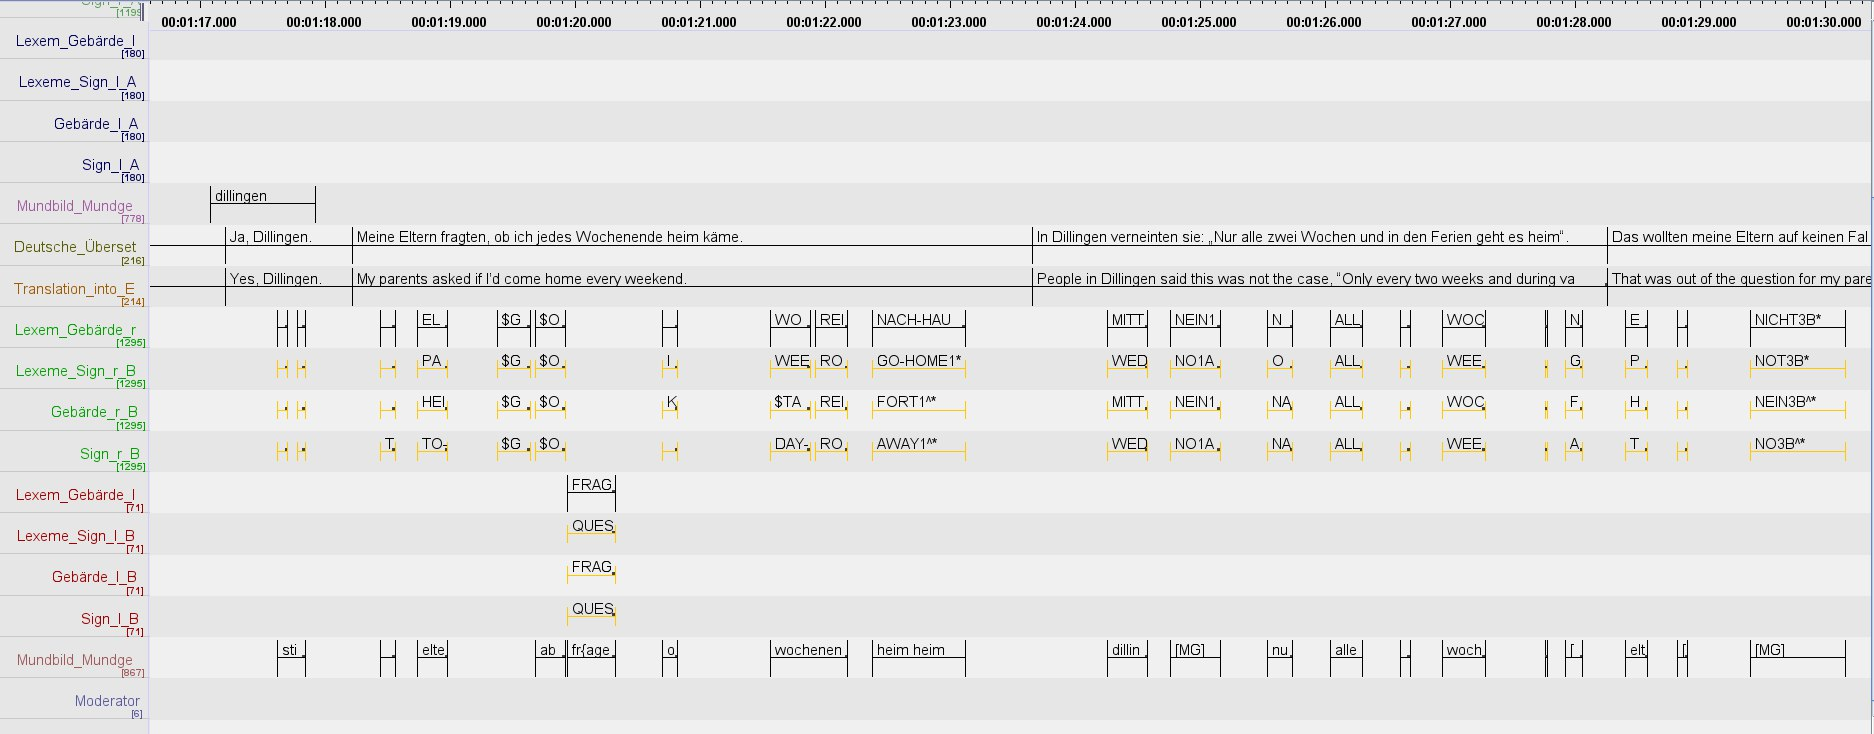
\includegraphics[width=14cm]{Bachelor CSAI thesis template/images/ELAN_example.jpg}
 \caption{Showing the structure of one of the EAF (English Annotated File)-files \cite{elan_example} inside the program ELAN. ELAN is a multimedia annotation tool used for multi-modality research \cite{sloetjes2017elan}. }
 \label{fig:elan_example}
\end{figure}

\subsubsection{Initial Translation}

The annotations divided into tiers are presented across a timeline. As can be seen in \autoref{fig:elan_example} these files are divided into $11$ different tiers, presented in both English and German due to accessibility \cite{konradoffentliches}. Take "Lexem\_Gebärde\_r\_A" for example, this tier is translated into English as "Lexeme\_Sign\_r\_A". The tiers present in the EAF-files, translated into English, are: "Time", "Sign\_l\_B", "Sign\_r\_B", "Lexeme\_Sign\_l\_B", "Lexeme\_Sign\_r\_B", 
"Translation\_into\_English\_B", "Sign\_l\_A", "Sign\_r\_A", "Lexeme\_Sign\_l\_A", "Lexeme\_Sign\_r\_A", and "Translation\_into\_English\_A" \cite{sloetjes2017elan}. The goal of this paper is to, through experimentation, show to what extent temporal data aids in the performance of a machine translation system for sign language glosses to text. For this purpose both the German Sign Language and the German Language were chosen respectively. Since the target language is German it was decided to use the original glosses and translations that were available in the corpus.

The initial translation of the glosses in the data set (i.e.: Sign\_l\_A to Translation\_into\_English) was conducted by contracted sign language translators, and interpreters \cite{konradoffentliches}. These researchers translated the data set word-for-word. Consequently, university students created coherent meaningful sentence like structures. Lastly these sentences were fed back into the system until the proper meaning was determined by the DGS-experts (\autoref{fig:uselesspipeline}) \cite{konradoffentliches}.

\begin{figure}[h]
 \centering 
 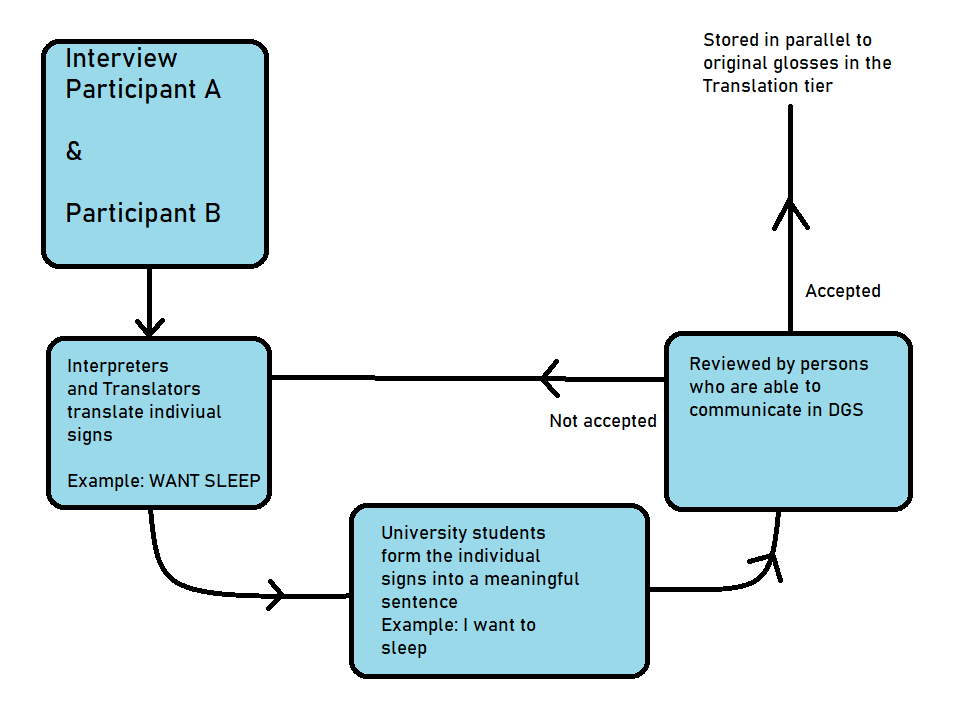
\includegraphics[width=14cm]{Bachelor CSAI thesis template/images/translation_pipeline.png}
 \caption{Showing the translation pipeline of the initial translation phase as conducted by the Institute for German Sign Language and Communication of the Deaf at Hamburg University. \cite{konradoffentliches} }
 \label{fig:uselesspipeline}
\end{figure}

\subsubsection{Lemmatisation and Gloss convention}

\subsubsection{Pre-Processing}
Using the ELAN-software $7$ of the $11$ tiers were selected and converted into a CSV-file. This creates $2$ distinct CSV-files that were consequently merged (\autoref{apx:first}). Due to being able to access the timeline in ELAN it is possible to extract the temporal features of a given annotation.
 



eaf files
elan
bpe - tokenizing preprocessing


\subsection{Method / Models}

different experiments
opennmt 
-removed white spaces and "nan" to equalize the parallel corpi
-bpe

features in tranlsation
bpe
sentencepiece



\section{Results}

\begin{table}
    
    \label{tab:results}
    \begin{tabular}{llrr}
        \toprule
                                                                  
        Word-Form                   &  Models                           &  BLEU                & TER    \\ 
        \midrule
        \multirow{3}{*}{Original}  &  Baseline                              &   \textbf{3.69}      &  \textbf{0.960} \\
                              & Temporal                                &   2.85               &  0.971 \\
                              & Vocal                                   &   2.03               &  1.000 \\
                              & Combined (Temporal + Vocal)             &   1.69               &  0.973 \\
    
        
    \end{tabular}
    \caption{SCHRIJF HIER NOG IETS}
\end{table}


\section{Discussion}

gebarentaal dialect neit meegomen

schrijf een stuk over wat er gebeurt als je dat hele ding standardised

\section{Conclusion}


\newpage
\bibliography{mybib}

\newpage
\appendix

\appendixsection{Merging Code} \label{apx:first}
\begin{lstlisting}[language=Python, caption=Section 6. Show is the Python code to merge the multiple CSV-files into one DataFrame.]
class create_file(object):
    def __init__(self, path="datasets/"):
        self.path = path
        self.inputs = listdir(str(path))
        self.dataframe = self.drop_empty()

    def clean_dataframe(self, dataset):
        """
        Load the dataset into a frame, delete the "Unnamed" column,
        and replace all instances of nothing with a numpy nan.
        Requires the numpy library.

        :param dataset: str, input name of the dataset.csv
        :return: dataframe, a cleaned dataframe with only used columns
        """
        dataframe = pd.read_csv(self.path + str(dataset), sep=",")  # Read into a frame
        dataframe = dataframe.loc[:, ~dataframe.columns.str.contains("^Unnamed")]  # Drop the "^Unnamed" column
        dataframe.replace("", np.nan, inplace=True)  # Replace the empty values with a nan

        return dataframe

    def merge(self):
        """
        The EAF-files consist of different persons, this functions merges those
        into one dataframe.

        :return: Dataframe. A merged dataframe consisting of all users.
        """
        combined = pd.DataFrame()
        for dataset in self.inputs:
            temp = self.clean_dataframe(dataset)

            # Normalize the column names into the translated versions.
            column_list = list(temp.columns)
            normalized_names = ["Time", "Right", "Mouth", "Translation", "Left"]
            # A dictionary is created with the corresponding column_list name and the normalized name
            translation_dict = {column_list[n]: normalized_names[n] for n in range(len(normalized_names))}
            temp = temp.rename(columns=translation_dict)

            # Combine the dataframes into one universal dataframe
            combined = combined.append(temp, ignore_index=True, sort=False)

        return combined

    def list_definer(self, input_list):
        """
        Finds the True instances in a list and stores their indexes.

        :param input_list: list, a list of True's and False's.
        :return: list, the list of indexes that were true in the input_list.
        """
        output_list = []
        # Looping over a enumerated input_list
        for number, element in enumerate(input_list):
            # If the element is True append the index else continue the loop
            if element:
                output_list.append(number)
            continue
        return output_list

    def drop_empty(self):
        """
        Dropping the empty rows from the dataset causing it to become more information packed.
        Downsides of this approach can be found in the Discussion of the written Thesis.

        :return: dataframe, a dataframe where there are no empty rows.
        """
        combined = self.merge()

        # Find the empty rows for each respective token (time excluded since it is always present).
        left_sign = set(self.list_definer(list(combined['Left'].isnull().values)))
        right_sign = set(self.list_definer(list(combined['Right'].isnull().values)))
        mouth_token = set(self.list_definer(list(combined['Mouth'].isnull().values)))

        # Find the intersection of these tokens.
        signs = left_sign.intersection(right_sign)
        empty_rows = signs.intersection(mouth_token)
        signs_missing = list(empty_rows)

        # Dropping the empty rows
        final_dataframe = combined.drop(signs_missing)

        return final_dataframe
\end{lstlisting}
 

